\appendix

\begin{frame}[noframenumbering, plain]{}
    Backup slides
\end{frame}

% XXX write those
\begin{frame}{MR signal derivation}
    
\end{frame}

\begin{frame}{Fourier Transform and MRI}
    
\end{frame}

\begin{frame}{More details on GRAPPA}
    
\end{frame}

\begin{frame}{Sparsity}
    
\end{frame}

\begin{frame}{Basis Pursuit}
    
\end{frame}

\begin{frame}{Sensitivity Maps}
    
\end{frame}

\begin{frame}{Noise model for MRI}
    
\end{frame}

\begin{frame}{Proximity operator}
    
\end{frame}

\begin{frame}{Convolutions}
    
\end{frame}

\begin{frame}{CNN}
    Convolutional Neural Network~(CNN): chain of Convolution + Nonlinearity.
\end{frame}

\begin{frame}{U-net}
    \begin{figure}
        \centering
        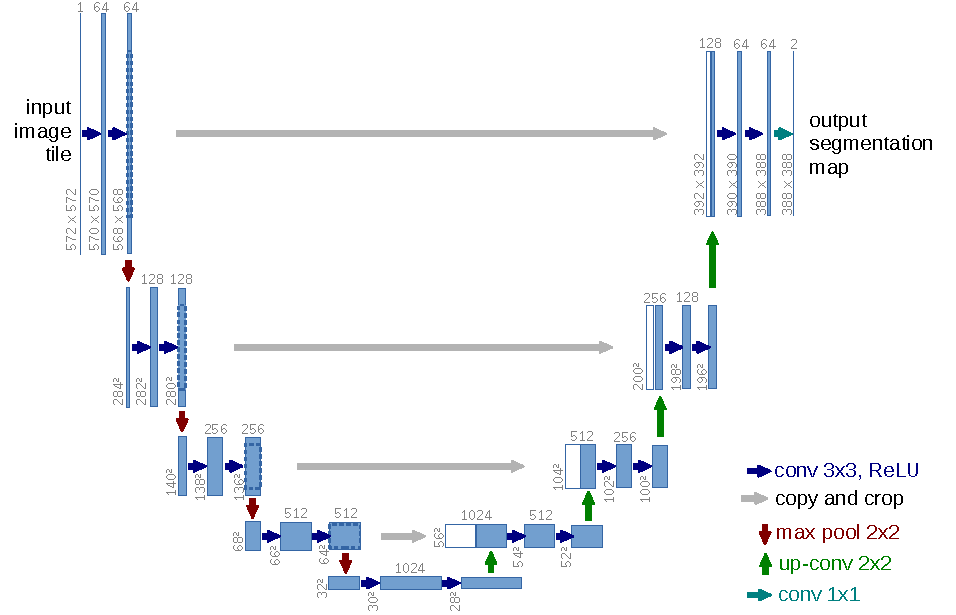
\includegraphics[height=0.6\textheight]{Figures/add_slides/unet_hires.pdf}
        \caption{Illustration from the original paper.\footfullcite{ronneberger2015u}}
    \end{figure}
\end{frame}

\begin{frame}{MWCNN}
    \begin{figure}
        \centering
        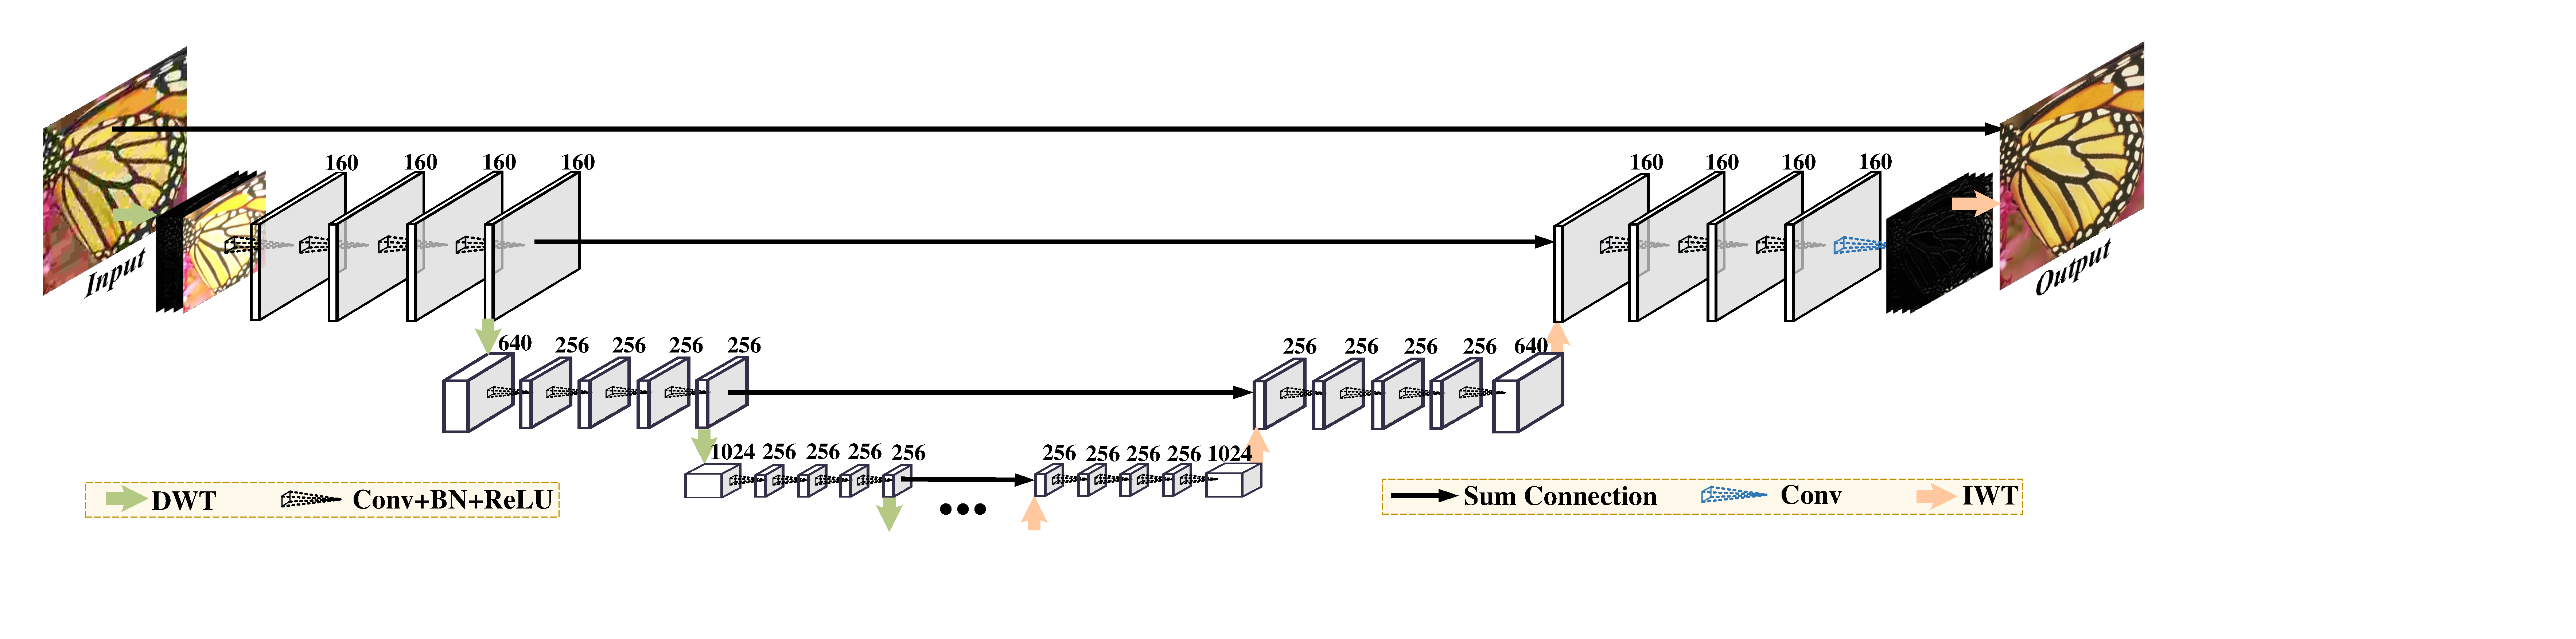
\includegraphics[width=\textwidth]{Figures/add_slides/mwcnn.pdf}
        \caption{Illustration from the original paper.\footfullcite{Liu2018}}
    \end{figure}
\end{frame}

\begin{frame}{fastMRI dataset}
    
\end{frame}

\begin{frame}{fastMRI challenge}
    
\end{frame}

\begin{frame}{autoMAP}
    
\end{frame}

\begin{frame}{XPDNet - ct'ed}
    
\end{frame}

\begin{frame}{PDNet \& Recurent Inference Machines}
    
\end{frame}

\begin{frame}{NC-PDNet - ct'ed}
    
\end{frame}

\begin{frame}{Image quality metrics}
    
\end{frame}

\begin{frame}{quasi-Newton methods}
    
\end{frame}

\begin{frame}{OPA - 1}
    
\end{frame}

\begin{frame}{OPA - 2}
    
\end{frame}

\begin{frame}{Jacobian-Free}
    
\end{frame}